\chapter{Introdução}
\label{chap:introducao}

Desde a pré-história, o ser humano tem a experiência de contar. Naquela época, o homem contava pequenas quantidades, 
como quantas pessoas tinham em seu bando ou quanto de alimento ele deveria coletar para sobreviver. Com o passar do 
tempo, o sistema numérico foi inventado para que pudéssemos trabalhar com valores cada vez maiores. 

\vspace{4mm}
\begin{figure}
  \centering
  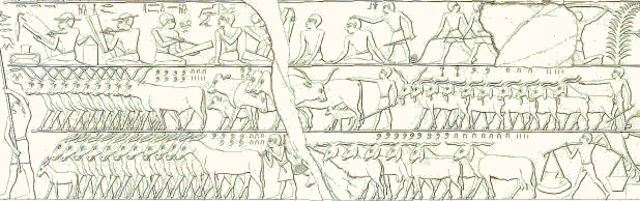
\includegraphics[width=\linewidth]{figuras/ancient_counting.png}
\end{figure} 
\vspace{2mm}

Quando pensávamos que contar não pudesse ficar mais difícil, os computadores surgem, abrindo novas discussões sobre a 
contagem. Entre elas, estavam como armazenar números em uma máquina, como fazer contas nesses aparelhos e até quanto 
poderíamos contar com a ajuda deles. E poucas décadas após essa invenção, a Internet é criada. 

Passamos, portanto, a ficar interessados em monitorar essa rede de computadores e para isso, tínhamos que descobrir 
quantas máquinas diferentes estavam acessando essa rede ou quem eram os aparelhos responsáveis pelo maior fluxo de dados. 
O principal desafio que surgiu nesse contexto, foi o alto volume de dados que precisavam ser processados em tempo real. 
E armazenar todos os dados localmente para em seguida, analisá-los deixou de ser viável devido à lentidão desse processo 
e ao elevado consumo de memória.

Estruturas de dados e algoritmos probabilísticos são uma forma de tentar contornar essa grande quantidade de informação. 
A ideia central é sacrificar a exatidão da resposta com o objetivo de consumir menos memória e tempo de processamento. 
Problemas que podem se beneficiar com soluções probabilísticas são, por exemplo, monitorar quantos usuários diferentes 
acessaram um site em um dado dia, contar quantas palavras distintas foram pesquisadas na última hora em uma plataforma 
de varejo ou armazenar quantas visualizações distintas um artigo teve. 

Uma característica comum desses problemas é que muitas vezes, suas respostas são métricas a serem utilizadas por outros 
sistemas com o intuito de se identificar falhas ou pontos de melhoria. No caso do monitoramento de quantas pessoas 
visitaram uma página web, uma forte queda nas visualizações pode ser um indício que um serviço esteja fora do ar. Nesse 
sentido, essas métricas não precisam ter necessariamente uma precisão de $100\%$, podendo apresentar um pequeno erro 
desde que sejam rapidademente computadas e leves de se armazenarem.

Por volta da década de~1970, Robert Morris tentou contar eventos cujo número de ocorrências não cabia na memória dos 
computadores da época~\citep{morris:78}. O \hyperref[chap:morris:algorithm]{algoritmo} proposto por ele serviu de 
inspiração para que outros autores conseguissem resolver problemas mais desafiadores, como a contagem distinta 
aproximada, cujo objetivo é estimar a quantidade de elementos distintos em um fluxo de dados. 

Alguns anos após Morris publicar o trabalho dele, a \hyperref[sec:flajolet-martin:algorithm]{$\pcounting$}, o primeiro 
algoritmo probabilístico que resolvia a contagem distinta aproximada, foi criada~\citep{flajolet:martin:85}. E a partir 
desse algoritmo, as soluções foram passando por melhorias, das quais podemos destacar a redução do consumo de memória, 
aumento da precisão e até mesmo o desenvolvimento de técnicas de demonstração que simplificavam o entendimento da razão 
desses algoritmos funcionarem.

Pouco tempo depois, as \hyperref[lab:chapter:04:01]{\asampling}, algoritmo que corrigia limitações da solução anterior, 
foram desenvolvidas~\citep{adptive:sampling:90}. Após uma década, a estrutura de dados 
\hyperref[sec:loglog:algorithm]{$\LOG$} é concebida, apresentando uma grande redução no consumo de 
memória~\citep{loglog:03}. E logo em seguida, o \hyperref[sec:loglog:hyperloglog]{$\HLOG$}, versão aperfeiçoada do 
$\LOG$, veio a público e se tornou uma das estruturas mais utilizadas para se resolver o problema da contagem distinta 
aproximada~\citep{hyperloglog:07}. Este texto, portanto, tem o objetivo de passar por essas soluções e apresentar 
comentários pertinentes de cada uma.

\vspace{2mm}
\begin{figure}
  \centering
  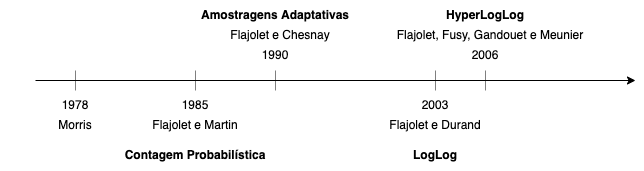
\includegraphics[width=\linewidth]{figuras/count_distinct_timeline.png}
\end{figure}  